\documentclass[]{article}
\usepackage{lmodern}
\usepackage{amssymb,amsmath}
\usepackage{ifxetex,ifluatex}
\usepackage{fixltx2e} % provides \textsubscript
\ifnum 0\ifxetex 1\fi\ifluatex 1\fi=0 % if pdftex
  \usepackage[T1]{fontenc}
  \usepackage[utf8]{inputenc}
\else % if luatex or xelatex
  \ifxetex
    \usepackage{mathspec}
  \else
    \usepackage{fontspec}
  \fi
  \defaultfontfeatures{Ligatures=TeX,Scale=MatchLowercase}
\fi
% use upquote if available, for straight quotes in verbatim environments
\IfFileExists{upquote.sty}{\usepackage{upquote}}{}
% use microtype if available
\IfFileExists{microtype.sty}{%
\usepackage{microtype}
\UseMicrotypeSet[protrusion]{basicmath} % disable protrusion for tt fonts
}{}
\usepackage[margin=2.54cm]{geometry}
\usepackage{hyperref}
\hypersetup{unicode=true,
            pdftitle={13: Time Series Analysis},
            pdfauthor={Environmental Data Analytics \textbar{} Kateri Salk},
            pdfborder={0 0 0},
            breaklinks=true}
\urlstyle{same}  % don't use monospace font for urls
\usepackage{color}
\usepackage{fancyvrb}
\newcommand{\VerbBar}{|}
\newcommand{\VERB}{\Verb[commandchars=\\\{\}]}
\DefineVerbatimEnvironment{Highlighting}{Verbatim}{commandchars=\\\{\}}
% Add ',fontsize=\small' for more characters per line
\usepackage{framed}
\definecolor{shadecolor}{RGB}{248,248,248}
\newenvironment{Shaded}{\begin{snugshade}}{\end{snugshade}}
\newcommand{\KeywordTok}[1]{\textcolor[rgb]{0.13,0.29,0.53}{\textbf{#1}}}
\newcommand{\DataTypeTok}[1]{\textcolor[rgb]{0.13,0.29,0.53}{#1}}
\newcommand{\DecValTok}[1]{\textcolor[rgb]{0.00,0.00,0.81}{#1}}
\newcommand{\BaseNTok}[1]{\textcolor[rgb]{0.00,0.00,0.81}{#1}}
\newcommand{\FloatTok}[1]{\textcolor[rgb]{0.00,0.00,0.81}{#1}}
\newcommand{\ConstantTok}[1]{\textcolor[rgb]{0.00,0.00,0.00}{#1}}
\newcommand{\CharTok}[1]{\textcolor[rgb]{0.31,0.60,0.02}{#1}}
\newcommand{\SpecialCharTok}[1]{\textcolor[rgb]{0.00,0.00,0.00}{#1}}
\newcommand{\StringTok}[1]{\textcolor[rgb]{0.31,0.60,0.02}{#1}}
\newcommand{\VerbatimStringTok}[1]{\textcolor[rgb]{0.31,0.60,0.02}{#1}}
\newcommand{\SpecialStringTok}[1]{\textcolor[rgb]{0.31,0.60,0.02}{#1}}
\newcommand{\ImportTok}[1]{#1}
\newcommand{\CommentTok}[1]{\textcolor[rgb]{0.56,0.35,0.01}{\textit{#1}}}
\newcommand{\DocumentationTok}[1]{\textcolor[rgb]{0.56,0.35,0.01}{\textbf{\textit{#1}}}}
\newcommand{\AnnotationTok}[1]{\textcolor[rgb]{0.56,0.35,0.01}{\textbf{\textit{#1}}}}
\newcommand{\CommentVarTok}[1]{\textcolor[rgb]{0.56,0.35,0.01}{\textbf{\textit{#1}}}}
\newcommand{\OtherTok}[1]{\textcolor[rgb]{0.56,0.35,0.01}{#1}}
\newcommand{\FunctionTok}[1]{\textcolor[rgb]{0.00,0.00,0.00}{#1}}
\newcommand{\VariableTok}[1]{\textcolor[rgb]{0.00,0.00,0.00}{#1}}
\newcommand{\ControlFlowTok}[1]{\textcolor[rgb]{0.13,0.29,0.53}{\textbf{#1}}}
\newcommand{\OperatorTok}[1]{\textcolor[rgb]{0.81,0.36,0.00}{\textbf{#1}}}
\newcommand{\BuiltInTok}[1]{#1}
\newcommand{\ExtensionTok}[1]{#1}
\newcommand{\PreprocessorTok}[1]{\textcolor[rgb]{0.56,0.35,0.01}{\textit{#1}}}
\newcommand{\AttributeTok}[1]{\textcolor[rgb]{0.77,0.63,0.00}{#1}}
\newcommand{\RegionMarkerTok}[1]{#1}
\newcommand{\InformationTok}[1]{\textcolor[rgb]{0.56,0.35,0.01}{\textbf{\textit{#1}}}}
\newcommand{\WarningTok}[1]{\textcolor[rgb]{0.56,0.35,0.01}{\textbf{\textit{#1}}}}
\newcommand{\AlertTok}[1]{\textcolor[rgb]{0.94,0.16,0.16}{#1}}
\newcommand{\ErrorTok}[1]{\textcolor[rgb]{0.64,0.00,0.00}{\textbf{#1}}}
\newcommand{\NormalTok}[1]{#1}
\usepackage{graphicx,grffile}
\makeatletter
\def\maxwidth{\ifdim\Gin@nat@width>\linewidth\linewidth\else\Gin@nat@width\fi}
\def\maxheight{\ifdim\Gin@nat@height>\textheight\textheight\else\Gin@nat@height\fi}
\makeatother
% Scale images if necessary, so that they will not overflow the page
% margins by default, and it is still possible to overwrite the defaults
% using explicit options in \includegraphics[width, height, ...]{}
\setkeys{Gin}{width=\maxwidth,height=\maxheight,keepaspectratio}
\IfFileExists{parskip.sty}{%
\usepackage{parskip}
}{% else
\setlength{\parindent}{0pt}
\setlength{\parskip}{6pt plus 2pt minus 1pt}
}
\setlength{\emergencystretch}{3em}  % prevent overfull lines
\providecommand{\tightlist}{%
  \setlength{\itemsep}{0pt}\setlength{\parskip}{0pt}}
\setcounter{secnumdepth}{0}
% Redefines (sub)paragraphs to behave more like sections
\ifx\paragraph\undefined\else
\let\oldparagraph\paragraph
\renewcommand{\paragraph}[1]{\oldparagraph{#1}\mbox{}}
\fi
\ifx\subparagraph\undefined\else
\let\oldsubparagraph\subparagraph
\renewcommand{\subparagraph}[1]{\oldsubparagraph{#1}\mbox{}}
\fi

%%% Use protect on footnotes to avoid problems with footnotes in titles
\let\rmarkdownfootnote\footnote%
\def\footnote{\protect\rmarkdownfootnote}

%%% Change title format to be more compact
\usepackage{titling}

% Create subtitle command for use in maketitle
\newcommand{\subtitle}[1]{
  \posttitle{
    \begin{center}\large#1\end{center}
    }
}

\setlength{\droptitle}{-2em}

  \title{13: Time Series Analysis}
    \pretitle{\vspace{\droptitle}\centering\huge}
  \posttitle{\par}
    \author{Environmental Data Analytics \textbar{} Kateri Salk}
    \preauthor{\centering\large\emph}
  \postauthor{\par}
      \predate{\centering\large\emph}
  \postdate{\par}
    \date{Spring 2019}


\begin{document}
\maketitle

\subsection{LESSON OBJECTIVES}\label{lesson-objectives}

\begin{enumerate}
\def\labelenumi{\arabic{enumi}.}
\tightlist
\item
  Describe the aspects of hierarchical models, fixed effects, and random
  effects
\item
  Choose and justify appropriate statistical models when time is an
  explanatory variable
\item
  Apply repeated measures ANOVA to datasets with temporal components
\end{enumerate}

\subsection{SET UP YOUR DATA ANALYSIS
SESSION}\label{set-up-your-data-analysis-session}

\begin{Shaded}
\begin{Highlighting}[]
\KeywordTok{getwd}\NormalTok{()}
\end{Highlighting}
\end{Shaded}

\begin{verbatim}
## [1] "C:/Users/Felipe/OneDrive - Duke University/1. DUKE/1. Ramos 2 Semestre/EOS-872 Env. Data Analytics/Environmental_Data_Analytics"
\end{verbatim}

\begin{Shaded}
\begin{Highlighting}[]
\KeywordTok{library}\NormalTok{(tidyverse)}
\CommentTok{#install.packages("lubridate")}
\KeywordTok{library}\NormalTok{(lubridate)}
\CommentTok{#install.packages("nlme")}
\KeywordTok{library}\NormalTok{(nlme)}
\CommentTok{#install.packages("lsmeans")}
\KeywordTok{library}\NormalTok{(lsmeans)}
\CommentTok{#install.packages("multcompView")}
\KeywordTok{library}\NormalTok{(multcompView)}

\NormalTok{PeterPaul.chem <-}\StringTok{ }\KeywordTok{read.csv}\NormalTok{(}\StringTok{"./Data/Processed/NTL-LTER_Lake_ChemistryPhysics_PeterPaul_Processed.csv"}\NormalTok{)}

\CommentTok{# Set date to date format}
\NormalTok{PeterPaul.chem}\OperatorTok{$}\NormalTok{sampledate <-}\StringTok{ }\KeywordTok{as.Date}\NormalTok{(PeterPaul.chem}\OperatorTok{$}\NormalTok{sampledate, }
                                               \DataTypeTok{format =} \StringTok{"%m/%d/%y"}\NormalTok{)}

\NormalTok{mytheme <-}\StringTok{ }\KeywordTok{theme_classic}\NormalTok{(}\DataTypeTok{base_size =} \DecValTok{14}\NormalTok{) }\OperatorTok{+}
\StringTok{  }\KeywordTok{theme}\NormalTok{(}\DataTypeTok{axis.text =} \KeywordTok{element_text}\NormalTok{(}\DataTypeTok{color =} \StringTok{"black"}\NormalTok{), }
        \DataTypeTok{legend.position =} \StringTok{"top"}\NormalTok{)}
\KeywordTok{theme_set}\NormalTok{(mytheme)}
\end{Highlighting}
\end{Shaded}

\subsection{HIERARCHICAL MODELS}\label{hierarchical-models}

\textbf{Hierarchical models,} or \textbf{mixed-effects models,} are a
type of linear model in which explanatory variables are given a model
whose parameters are also estimated by the data. The coefficients
associated with explanatory variables thus may not be a single value but
instead be sampled from a distribution, called the hyper-distribution,
which is defined by the modeler. The advantage of the hierarchical model
is that it builds capacity to describe multiple layers of stochasticity,
which enables accounting of all aspects of uncertainty in a system.
Specifically, we can separately model the process of interest and the
sampling process.

The coefficients of a hierarchical model are divided into two
categories: \textbf{fixed effects} and \textbf{random effects.} A
\textbf{fixed effect} is a factor whose levels are experimentally
determined or whose interest lies in the effects of each level (e.g.,
covariates, treatments, interactions). A \textbf{random effect} is a
factor whose levels are sampled from a larger population, or whose
interest lies in the variation among them rather than the specific
effect of each level. In choosing whether you are dealing with a fixed
or a random effect, consider the following questions:

\begin{itemize}
\item
  Do you have a particular interest in the studied factor level? FRA:
  all fixe effect
\item
  Have you included all possible levels in the study? FRA: all, fixed
  effect
\item
  Do you have interest in the variance among levels? Parece que random
  effect.
\item
  Do you have interest in generalizing to factor levels that you did not
  study? Random effect
\end{itemize}

One common variable in hierarchical models is \textbf{time.} Time can be
a complicated explanatory variable, as it can act as either a fixed or a
random effect depending on the study design and research question. Due
to \textbf{temporal autocorrelation,} conditions measured at a single
site will be highly influenced by the conditions preceding the sampling
date. Therefore, two samples taken in relatively close temporal
proximity may not necessarily be independent of one another. Treating
time as a random effect will account for temporal trends in observations
(e.g., diel or seasonal patterns) that may not be of interest for your
study. FRA: this violates the indepedent assump.

Another common variable in hierarchical models is \textbf{space.} In
many situations, we may want to infer conditions beyond the sites that
we have sampled. By treating space as a random variable, we may be able
to extrapolate conditions of the response variable across a spatial
gradient. FRA: we have some points but want to generalize
--\textgreater{} random effects.

\subsection{REPEATED MEASUREMENTS AND
AUTOCORRELATION}\label{repeated-measurements-and-autocorrelation}

In many situations where monitoring is conducted, samples taken
repeatedly at a given site may not be considered truly independent. The
conditions present on a given day may be dependent on conditions present
earlier in time. This is clearly an issue for the way we might
traditionally think of experimental design and statistical independence,
but this type of study design is often of interest in the field of
environmental science. We can set up models to consider autocorrelation
of time within a given place. One example of this type of model is a
\textbf{repeated measures ANOVA}.

Let's think about the situation of temperature monitoring in the
NTL-LTER lake sites, Peter and Paul Lakes. We might be interested to
know whether surface temperatures in the summer have increased over time
in response to climate change. However, we know that (a) temperature
conditions on a given date are dependent on conditions earlier in the
season, and (b) there is considerable variability across the summer
season within a year (i.e., cooler temperatures occurring in June
vs.~August). We can set up a hierarchical model to deal with the
autocorrelation by date as well as the variability associated with
seasonality.

Let's wrangle our data and visualize a preliminary relationship between
our variables of interest.

\begin{Shaded}
\begin{Highlighting}[]
\NormalTok{PeterPaul.summertemp <-}\StringTok{ }
\StringTok{  }\NormalTok{PeterPaul.chem }\OperatorTok
\StringTok{  }\KeywordTok{select}\NormalTok{(lakename}\OperatorTok{:}\NormalTok{temperature_C) }\OperatorTok
\StringTok{  }\CommentTok{#filter for Julian days in June-August and surface measurements}
\StringTok{  }\KeywordTok{filter}\NormalTok{(daynum }\OperatorTok{>}\StringTok{ }\DecValTok{151} \OperatorTok{&}\StringTok{ }\NormalTok{daynum }\OperatorTok{<}\StringTok{ }\DecValTok{243} \OperatorTok{&}\StringTok{ }\NormalTok{depth }\OperatorTok{==}\StringTok{ }\DecValTok{0}\NormalTok{ ) }\OperatorTok\StringTok{ }\CommentTok{# just a period of time and just surface.}
\StringTok{  }\CommentTok{#add a "week" column to represent seasonality}
\StringTok{  }\KeywordTok{mutate}\NormalTok{(}\DataTypeTok{Week =} \KeywordTok{week}\NormalTok{(sampledate)) }\OperatorTok
\StringTok{  }\CommentTok{#code won't work if there are NAs}
\StringTok{  }\KeywordTok{na.exclude}\NormalTok{() }\CommentTok{# careful that you dont erase useful data.}

\KeywordTok{ggplot}\NormalTok{(PeterPaul.summertemp, }\KeywordTok{aes}\NormalTok{(}\DataTypeTok{x =}\NormalTok{ sampledate, }\DataTypeTok{y =}\NormalTok{ temperature_C, }\DataTypeTok{color =}\NormalTok{ lakename)) }\OperatorTok{+}
\StringTok{  }\KeywordTok{geom_point}\NormalTok{() }\OperatorTok{+}
\StringTok{  }\KeywordTok{scale_color_manual}\NormalTok{(}\DataTypeTok{values =} \KeywordTok{c}\NormalTok{(}\StringTok{"#7fcdbb"}\NormalTok{, }\StringTok{"#253494"}\NormalTok{))}
\end{Highlighting}
\end{Shaded}

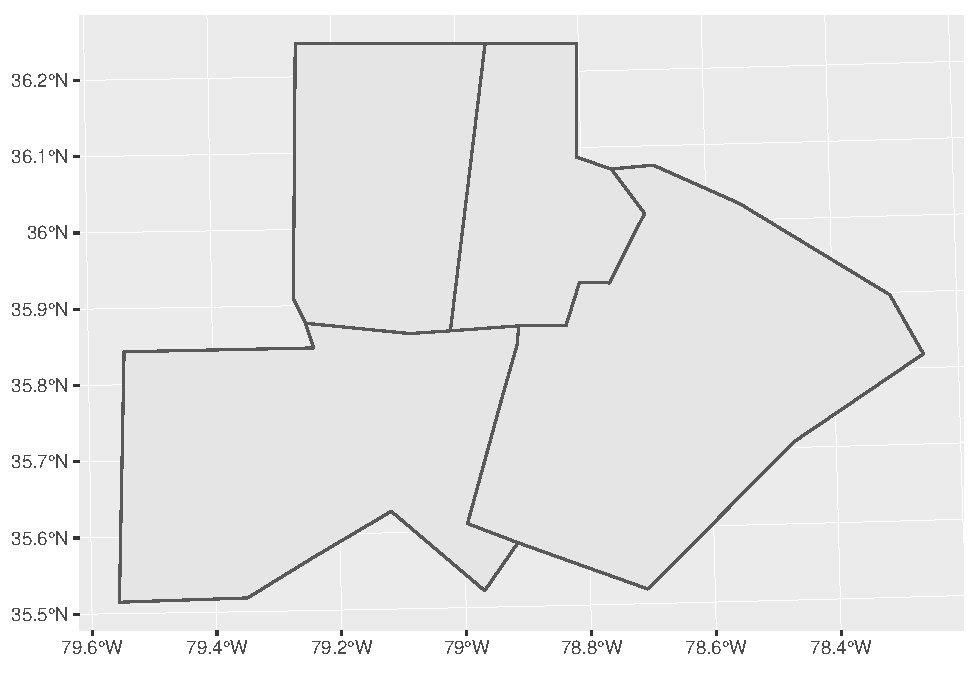
\includegraphics{13_TimeSeries_files/figure-latex/unnamed-chunk-2-1.pdf}

Next, we will determine the degree of temporal autocorrelation in our
dataset. We will use the package \texttt{nlme} for our analyses. Another
good package for running hierarchical, or mixed-effects, models is
\texttt{lme4}. For the basic types of hierarchical models, these
packages have about the same functionality.

\begin{Shaded}
\begin{Highlighting}[]
\CommentTok{# Determine autocorrelation in residuals}
\NormalTok{TempTest.auto <-}\StringTok{ }\KeywordTok{lme}\NormalTok{(}\DataTypeTok{data =}\NormalTok{ PeterPaul.summertemp,}
\NormalTok{                     temperature_C }\OperatorTok{~}\StringTok{ }\NormalTok{sampledate }\OperatorTok{*}\StringTok{ }\NormalTok{lakename, }
                     \DataTypeTok{random =} \OperatorTok{~}\DecValTok{1}\OperatorTok{|}\NormalTok{Week)}
\NormalTok{TempTest.auto}
\end{Highlighting}
\end{Shaded}

\begin{verbatim}
## Linear mixed-effects model fit by REML
##   Data: PeterPaul.summertemp 
##   Log-restricted-likelihood: -1841.595
##   Fixed: temperature_C ~ sampledate * lakename 
##                   (Intercept)                    sampledate 
##                  2.061909e+01                  8.816467e-05 
##            lakenamePeter Lake sampledate:lakenamePeter Lake 
##                  1.093329e-01                  2.204779e-06 
## 
## Random effects:
##  Formula: ~1 | Week
##         (Intercept) Residual
## StdDev:    1.588171 1.941958
## 
## Number of Observations: 863
## Number of Groups: 14
\end{verbatim}

\begin{Shaded}
\begin{Highlighting}[]
\CommentTok{# what the variability is among the weeks. That is why it gives a StdDev. (the random effect).}
\CommentTok{# Fixed effects gives coef.}

\KeywordTok{summary}\NormalTok{(TempTest.auto) }\CommentTok{# esto lo puse yo}
\end{Highlighting}
\end{Shaded}

\begin{verbatim}
## Linear mixed-effects model fit by REML
##  Data: PeterPaul.summertemp 
##        AIC      BIC    logLik
##   3695.189 3723.724 -1841.595
## 
## Random effects:
##  Formula: ~1 | Week
##         (Intercept) Residual
## StdDev:    1.588171 1.941958
## 
## Fixed effects: temperature_C ~ sampledate * lakename 
##                                   Value Std.Error  DF  t-value p-value
## (Intercept)                   20.619095 0.5218706 846 39.50998  0.0000
## sampledate                     0.000088 0.0000262 846  3.36343  0.0008
## lakenamePeter Lake             0.109333 0.4298095 846  0.25438  0.7993
## sampledate:lakenamePeter Lake  0.000002 0.0000372 846  0.05924  0.9528
##  Correlation: 
##                               (Intr) smpldt lknmPL
## sampledate                    -0.553              
## lakenamePeter Lake            -0.410  0.671       
## sampledate:lakenamePeter Lake  0.390 -0.704 -0.952
## 
## Standardized Within-Group Residuals:
##         Min          Q1         Med          Q3         Max 
## -3.23374297 -0.61443099  0.05643875  0.61436794  2.96775134 
## 
## Number of Observations: 863
## Number of Groups: 14
\end{verbatim}

\begin{Shaded}
\begin{Highlighting}[]
\CommentTok{# }
\KeywordTok{ACF}\NormalTok{(TempTest.auto)}
\end{Highlighting}
\end{Shaded}

\begin{verbatim}
##    lag         ACF
## 1    0  1.00000000
## 2    1  0.42324818
## 3    2  0.04801177
## 4    3 -0.04227307
## 5    4 -0.08775368
## 6    5 -0.07702138
## 7    6 -0.13094473
## 8    7 -0.10997063
## 9    8 -0.02905440
## 10   9 -0.02826303
## 11  10 -0.01730103
## 12  11 -0.01476535
## 13  12 -0.04397958
## 14  13 -0.04780381
## 15  14 -0.05377938
## 16  15  0.01680037
## 17  16  0.02257738
## 18  17 -0.03976543
## 19  18 -0.09594045
\end{verbatim}

\begin{Shaded}
\begin{Highlighting}[]
\CommentTok{# position 2 --> 42.3%}
\end{Highlighting}
\end{Shaded}

This model structure should look familiar, with a typical linear model
structure and dataframe defined. The addition here is that we have
defined Week as a random variable. Essentially, we are interested not in
the specific effects of each week but in the variability among weeks, so
we have defined it as a random effect (essentially coming from a larger
distribution of seasonal variability). The \textasciitilde{}1 statement
indicates that each week has its own intercept in the model. From here,
we want to take the first order correlation to specify our
autocorrelation structure. From the ACF output, we take the 2nd value
(the innermost group level) to define the degree of autocorrelation.
This number will always fall between 0 and 1. Notice that there is a
fairly large degree of autocorrelation in our variables.

We will now create a repeated measures ANOVA model now that we have
defined our autocorrelation structure. The way we have set up this
model, we are considering temporal autocorrelation within the levels of
Week, and we have retained Week as a random effect.

The correlation statement in the model is defined as follows:
\texttt{correlation\ =\ structure(form\ =\ \textasciitilde{}\ time\ \textbar{}\ subjvar)},
where structure is the autocorrelative structure (options in
\texttt{?corClasses}), time is the temporal variable, and subjvar is the
variable for experimental units.

\begin{Shaded}
\begin{Highlighting}[]
\NormalTok{TempTest.mixed <-}\StringTok{ }\KeywordTok{lme}\NormalTok{(}\DataTypeTok{data =}\NormalTok{ PeterPaul.summertemp,}
\NormalTok{                     temperature_C }\OperatorTok{~}\StringTok{ }\NormalTok{sampledate }\OperatorTok{*}\StringTok{ }\NormalTok{lakename, }
                     \DataTypeTok{random =} \OperatorTok{~}\DecValTok{1}\OperatorTok{|}\NormalTok{Week,}
                     \CommentTok{#specify autocorrelation structure of order 1 (this is the 42.3%)}
                     \CommentTok{#sampledate is duplicated in some cases, so need to split up by lake. }
                     \CommentTok{#FRA: This is only beacuse R doesnt like  that the sample were taken the same time.}
                     \DataTypeTok{correlation =} \KeywordTok{corAR1}\NormalTok{(}\DataTypeTok{form =} \OperatorTok{~}\StringTok{ }\NormalTok{sampledate}\OperatorTok{/}\NormalTok{lakename}\OperatorTok{|}\NormalTok{Week, }\DataTypeTok{value =} \FloatTok{0.423}\NormalTok{), }
                     \CommentTok{# we put manually the 0.423}
                     \CommentTok{#define method as restricted maximum likelihood}
                     \DataTypeTok{method =} \StringTok{"REML"}\NormalTok{)}
\KeywordTok{summary}\NormalTok{(TempTest.mixed)}
\end{Highlighting}
\end{Shaded}

\begin{verbatim}
## Linear mixed-effects model fit by REML
##  Data: PeterPaul.summertemp 
##        AIC      BIC    logLik
##   3678.638 3711.928 -1832.319
## 
## Random effects:
##  Formula: ~1 | Week
##         (Intercept) Residual
## StdDev:    1.618912 1.930645
## 
## Correlation Structure: ARMA(1,0)
##  Formula: ~sampledate/lakename | Week 
##  Parameter estimate(s):
##      Phi1 
## 0.5910308 
## Fixed effects: temperature_C ~ sampledate * lakename 
##                                   Value Std.Error  DF  t-value p-value
## (Intercept)                   20.466650 0.5323160 846 38.44831  0.0000
## sampledate                     0.000099 0.0000266 846  3.73751  0.0002
## lakenamePeter Lake             0.072415 0.4409492 846  0.16423  0.8696
## sampledate:lakenamePeter Lake  0.000005 0.0000379 846  0.12217  0.9028
##  Correlation: 
##                               (Intr) smpldt lknmPL
## sampledate                    -0.554              
## lakenamePeter Lake            -0.409  0.669       
## sampledate:lakenamePeter Lake  0.389 -0.701 -0.953
## 
## Standardized Within-Group Residuals:
##         Min          Q1         Med          Q3         Max 
## -3.23677606 -0.59679953  0.07085816  0.63629846  3.02528688 
## 
## Number of Observations: 863
## Number of Groups: 14
\end{verbatim}

\begin{Shaded}
\begin{Highlighting}[]
\CommentTok{#Results: Random we got a stddev. Fixed effects: lakenamePeter Lake coef --> no diff between lakes. }
\CommentTok{# The interaction is also not significant.}

\CommentTok{# Compare the random effects model with the fixed effects model}
\NormalTok{TempTest.fixed <-}\StringTok{ }\KeywordTok{gls}\NormalTok{(}\DataTypeTok{data =}\NormalTok{ PeterPaul.summertemp,}
\NormalTok{                      temperature_C }\OperatorTok{~}\StringTok{ }\NormalTok{sampledate }\OperatorTok{*}\StringTok{ }\NormalTok{lakename, }
                      \DataTypeTok{method =} \StringTok{"REML"}\NormalTok{)}
\KeywordTok{summary}\NormalTok{(TempTest.fixed)}
\end{Highlighting}
\end{Shaded}

\begin{verbatim}
## Generalized least squares fit by REML
##   Model: temperature_C ~ sampledate * lakename 
##   Data: PeterPaul.summertemp 
##        AIC      BIC    logLik
##   4019.694 4043.473 -2004.847
## 
## Coefficients:
##                                   Value Std.Error  t-value p-value
## (Intercept)                   20.800214 0.3770183 55.17031  0.0000
## sampledate                     0.000085 0.0000326  2.59341  0.0097
## lakenamePeter Lake             0.085356 0.5344819  0.15970  0.8732
## sampledate:lakenamePeter Lake  0.000006 0.0000463  0.12712  0.8989
## 
##  Correlation: 
##                               (Intr) smpldt lknmPL
## sampledate                    -0.951              
## lakenamePeter Lake            -0.705  0.671       
## sampledate:lakenamePeter Lake  0.670 -0.704 -0.951
## 
## Standardized residuals:
##        Min         Q1        Med         Q3        Max 
## -3.5435857 -0.6593598  0.1113940  0.6964839  2.4025400 
## 
## Residual standard error: 2.415319 
## Degrees of freedom: 863 total; 859 residual
\end{verbatim}

\begin{Shaded}
\begin{Highlighting}[]
\CommentTok{# little diff results but same conclusions}
\CommentTok{# why did we wanto to use random effect? --> We now there is variability. why dont use }
\CommentTok{# that for our advantage.}

\KeywordTok{anova}\NormalTok{(TempTest.mixed, TempTest.fixed)}
\end{Highlighting}
\end{Shaded}

\begin{verbatim}
##                Model df      AIC      BIC    logLik   Test  L.Ratio
## TempTest.mixed     1  7 3678.638 3711.928 -1832.319                
## TempTest.fixed     2  5 4019.694 4043.473 -2004.847 1 vs 2 345.0563
##                p-value
## TempTest.mixed        
## TempTest.fixed  <.0001
\end{verbatim}

\begin{Shaded}
\begin{Highlighting}[]
\CommentTok{# The lower the AIC, the better.}
\CommentTok{# The p-value tells us whether those models have a significantly different fit}

\CommentTok{# FRA: the models and signif diff and the mixed is better (AIC)}

\CommentTok{# Post-hoc test}
\CommentTok{# This will yield groupings of temperature by lake for the average date value}
\NormalTok{TempTest.posthoc =}\StringTok{ }\KeywordTok{lsmeans}\NormalTok{(TempTest.mixed, }\OperatorTok{~}\StringTok{ }\NormalTok{sampledate }\OperatorTok{*}\StringTok{ }\NormalTok{lakename)}
\KeywordTok{cld}\NormalTok{(TempTest.posthoc, }\DataTypeTok{alpha =} \FloatTok{0.05}\NormalTok{, }\DataTypeTok{Letters =}\NormalTok{ letters, }\DataTypeTok{adjust =} \StringTok{"tukey"}\NormalTok{)}
\end{Highlighting}
\end{Shaded}

\begin{verbatim}
##  sampledate lakename   lsmean    SE df lower.CL upper.CL .group
##       10989 Paul Lake    21.6 0.443 13     20.4     22.7  a    
##       10989 Peter Lake   21.7 0.443 13     20.6     22.8  a    
## 
## d.f. method: containment 
## Confidence level used: 0.95 
## Conf-level adjustment: sidak method for 2 estimates 
## significance level used: alpha = 0.05
\end{verbatim}

\begin{Shaded}
\begin{Highlighting}[]
\CommentTok{# FRA: you want this is there is a signif diff between groups. Something about groups.}


\CommentTok{# display our final relationship}
\KeywordTok{ggplot}\NormalTok{(PeterPaul.summertemp, }\KeywordTok{aes}\NormalTok{(}\DataTypeTok{x =}\NormalTok{ sampledate, }\DataTypeTok{y =}\NormalTok{ temperature_C, }\DataTypeTok{color =}\NormalTok{ lakename)) }\OperatorTok{+}
\StringTok{  }\KeywordTok{geom_point}\NormalTok{() }\OperatorTok{+}
\StringTok{  }\KeywordTok{scale_color_manual}\NormalTok{(}\DataTypeTok{values =} \KeywordTok{c}\NormalTok{(}\StringTok{"#7fcdbb"}\NormalTok{, }\StringTok{"#253494"}\NormalTok{)) }\OperatorTok{+}
\StringTok{  }\KeywordTok{geom_abline}\NormalTok{(}\DataTypeTok{intercept =} \FloatTok{20.47}\NormalTok{, }\DataTypeTok{slope =} \FloatTok{0.0001}\NormalTok{) }\CommentTok{#rounded coeff.}
\end{Highlighting}
\end{Shaded}

\includegraphics{13_TimeSeries_files/figure-latex/unnamed-chunk-4-1.pdf}

Question: How would you interpret the collective results of your mixed
effects model in the context of the study question?

\begin{quote}
ANSWER:
\end{quote}


\end{document}
